% !TeX program = xelatex

%%% Загружаем заголовочный файл, который хранит все настройки и все
%%% подгружаемые пакеты
\newcommand{\No}{\textnumero}

\PassOptionsToPackage{hidelinks}{hyperref}


%%% Здесь выбираются необходимые графы
\documentclass[russian,utf8,pointsection,nocolumnsxix,nocolumnxxxi,nocolumnxxxii]{eskdtext}
\usepackage{fontspec}
\defaultfontfeatures{Mapping=tex-text}

%%% Чтобы работал eskdx и другие пакеты
\usepackage{xecyr}

%%% Шрифты и кодировки
\usepackage{xunicode,xltxtra}
\usepackage{listings}
\usepackage{longtable}
\usepackage{caption}

%%% Русский текст
\setmainfont{Times New Roman}
\setromanfont{Times New Roman}
\setsansfont{Times New Roman}
\setmonofont{Times New Roman}

%%% Математика
\usepackage{amsmath,amssymb}

%%% Символ градуса
\usepackage{gensymb}

%%% Перенос составных слов
\XeTeXcharclass `\- 24
\XeTeXinterchartoks 24 0 ={\hskip\z@skip}
\XeTeXinterchartoks 0 24 ={\nobreak}

%%% Подпись «Рисунок» вместо «рис. 1»
\addto{\captionsrussian}{\renewcommand{\figurename}{Рисунок}}

%%% Убираем точки после цифр в заголовках
\def\russian@capsformat{%
	\def\postchapter{\@aftersepkern}%
	\def\postsection{\@aftersepkern}%
	\def\postsubsection{\@aftersepkern}%
	\def\postsubsubsection{\@aftersepkern}%
	\def\postparagraph{\@aftersepkern}%
	\def\postsubparagraph{\@aftersepkern}%
}

\sloppy

%%% Графика, ссылки, ToC
\usepackage{graphicx,float,url}
\setcounter{tocdepth}{3}

%%% Гиперссылки
\usepackage{hyperref}

%%% Заголовки разделов
\usepackage{titlesec}
\titleformat{\section}[block]{\normalfont\Large\bfseries}{\thesection}{1em}{}
\titlespacing*{\section}{1cm}{14pt}{8pt}

\titleformat{\subsection}[block]{\normalfont\large\bfseries}{\thesubsection}{1em}{}
\titlespacing*{\subsection}{1cm}{12pt}{6pt}

\titleformat{\subsubsection}[block]{\normalfont\normalsize\bfseries}{\thesubsubsection}{1em}{}
\titlespacing*{\subsubsection}{1cm}{10pt}{4pt}

%%% === Патч нумерации subsubsection ===
\usepackage{etoolbox}               % подтягиваем \preto

% 1) объявляем счётчик
\newcounter{subsubsectcount}

% 2) перед каждым \section: разрыв страницы + сброс нашего счётчика
\preto\section{%
	\clearpage
	\setcounter{subsubsectcount}{0}%
}

% 3) сохраняем оригинальную команду
%\let\origsubsubsection\subsubsection
%
%% 4) переопределяем логику
%\renewcommand{\subsubsection}[1]{%
%	\stepcounter{subsubsectcount}%
%	\ifnum\value{subsubsectcount}>6
%	% после 5-й — звёздочная версия (без номера и без ToC)
%	\origsubsubsection*{#1}%
%	\else
%	% первые 5 — как обычно
%	\origsubsubsection{#1}%
%	\fi
%}
%%% ====================================

%%% 1) Подключаем пакеты (у вас уже есть)
\usepackage{listings}
\usepackage{xcolor}
\usepackage{fontspec}
\setmonofont{JetBrains Mono}

%%% 1) Базовый стиль
\lstdefinestyle{custom}{
	basicstyle=\ttfamily\fontsize{10pt}{12pt}\selectfont,
	frame=single,
	backgroundcolor=\color{gray!10},
	keywordstyle=\bfseries\color{blue!70!black},
	commentstyle=\itshape\color{gray!60},
	stringstyle=\color{red!70!black},
	numbers=left,
	numberstyle=\tiny\color{gray!50},
	xleftmargin=2em,
	xrightmargin=2em,
	showstringspaces=false,
}

%%% 2) Язык TypeScript/TSX
\lstdefinelanguage{TypeScript}{
	sensitive=true,          % регистрозависимый
	breaklines=true,         % перенос длинных строк
	morekeywords={%
		abstract,any,as,asserts,async,await,boolean,break,case,catch,class,const,continue,%
		debugger,declare,default,delete,do,else,enum,export,extends,false,finally,for,%
		from,function,get,if,implements,import,in,instanceof,interface,let,module,namespace,%
		never,new,null,number,of,package,private,protected,public,readonly,require,return,%
		set,static,string,super,switch,symbol,this,throw,true,try,type,typeof,undefined,%
		unique,unknown,var,void,while,with,yield%
	},
	morecomment=[l]{//},
	morecomment=[s]{/*}{*/},
	morestring=[b]",
	morestring=[b]',
	alsoletter={<,>,/},
	moredelim=**[is][\color{blue!50!black}]{<}{>},
	literate={%
		{<}{{$<$}}1
		{>}{{$>$}}1
		{/}{{$/$}}1
	}%
}  % <-- убедитесь, что закрывающая } на месте

%%% 3) Стиль для TS/TSX
\lstdefinestyle{tscustom}{
style=custom,
language=TypeScript,
tabsize=2,
breakatwhitespace=false,
columns=fullflexible,
keepspaces=true,
breakautoindent=true,
breakindent=1em,
postbreak=\mbox{\textcolor{gray}{$\hookrightarrow$}\space},
}

%%% 4) Устанавливаем tscustom по умолчанию
\lstset{style=tscustom}

\usepackage[parentracker=true,
backend=biber,
hyperref=false,
bibencoding=utf8,
style=numeric-comp,
language=auto,
autolang=other,
citestyle=gost-numeric,
defernumbers=true,
bibstyle=gost-numeric,
sorting=none,
]{biblatex}
\addbibresource{bibliography.bib}


\usepackage{subcaption}
\usepackage{booktabs}

\setlength{\parindent}{1cm}

\usepackage{enumitem}
% Для первого уровня списка enumerate
\setlist[enumerate,1]{label=\arabic*), leftmargin=1cm}

% Для второго уровня (если нужно)
\setlist[enumerate,2]{label=\alph*), leftmargin=1cm}

% Для itemize (если нужно настроить)
\setlist[itemize]{leftmargin=1cm}

%%% Настройка основного шрифта и интервала
%\usepackage{setspace} % Добавляем пакет для интервалов
%\onehalfspacing       % Полуторный межстрочный интервал
%\renewcommand{\normalsize}{\fontsize{14pt}{16pt}\selectfont} % 14pt с интервалом 1.5

%%% Абзацный отступ (уже есть, но дублируем для надежности)
\setlength{\parindent}{1cm} 

%%% Настройка отступов для заголовков
\usepackage{titlesec}
% Section: 1cm слева, 14pt сверху, 8pt снизу
\titleformat{\section}[block]{\normalfont\bfseries}{\thesection}{0.5em}{}
\titlespacing*{\section}{1cm}{14pt}{8pt}

% Subsection
\titleformat{\subsection}[block]{\normalfont\bfseries}{\thesubsection}{0.5em}{}
\titlespacing*{\subsection}{1cm}{12pt}{6pt}

% Subsubsection
\titleformat{\subsubsection}[block]{\normalfont\bfseries}{\thesubsubsection}{0.5em}{}
\titlespacing*{\subsubsection}{1cm}{10pt}{4pt}

%%% Убираем заголовок "Содержание" у оглавления
\makeatletter
\renewcommand{\tableofcontents}{%
    \@starttoc{toc}%
}
\makeatother


\newfontfamily\jetbrainsmono{JetBrains Mono}[
  Scale=1.0,
  ItalicFont={JetBrains Mono Italic},
  BoldFont={JetBrains Mono Bold},
  BoldItalicFont={JetBrains Mono Bold Italic},
]

\usepackage{titletoc}
% ----------------------------
% 1) Настройка секций
% ----------------------------
\titlecontents{section}% уровень — section
  [0.5cm]                        % отступ слева
  {}                           % код перед строкой
  {\contentslabel{0.8em}\hspace{0cm}} % нумерация шириной 1.8em + 0.4em после неё
  {}                           % для ненумерованных
  {\titlerule*[0.5em]{.}\contentspage}% dot-линия (0.5em между точками) + номер страницы
  []

% ----------------------------
% 2) (по желанию) subsection/subsubsection
% ----------------------------
\titlecontents{subsection}
  [0.8cm]                      % дополнительный отступ для вложенности
  {}%
  {\contentslabel{1.0em}\hspace{0.5cm}}
  {}%
  {\titlerule*[0.3em]{.}\contentspage}
  []

\titlecontents{subsubsection}
  [1.8cm]
  {}%
  {\contentslabel{2em}\hspace{0.3cm}}
  {}%
  {\titlerule*[0.2em]{.}\contentspage}
  []
  
\usepackage{caption,newfloat}
\DeclareFloatingEnvironment[
  fileext=lol,
  name=Листинг,
  listname=Список\,листингов
]{listing}

% 1) формат «Листинг <номер> – »
\DeclareCaptionLabelFormat{dash}{#1~#2~–~}

% 2) настраиваем подписи именно для окружения listing
\captionsetup[lstlisting]{%
  labelformat=dash,    % наш «–» вместо «:»
  labelsep=none,       % разделитель мы уже вставили в labelformat
  font=normal,          % маленький шрифт, как для рисунков/таблиц
  justification=raggedright, % выравнивание по левому краю
  singlelinecheck=false % даже в одну строку выравнивать по raggedright
}

\usepackage[hidelinks]{hyperref}

%%% Загружаем настройки пакета eskdx, там нужно заполнить информацию
%%% о документе - ФИО авторов, название документов и т.п.
%%% Название документа
\ESKDtitle{ Название документа }
\ESKDdocName{ Название дипломной работы  Название дипломной работы     }

\renewcommand{\ESKDcolumnXfIIname}{Руковод.}
\renewcommand{\ESKDcolumnXfIVname}{Консул.}
\renewcommand{\ESKDcolumnXfVIname}{Зав. Каф.}

\ESKDauthor{Иванов А. Б.}
\ESKDchecker{Мельников А.Б. }
\ESKDnormContr{ Н.Кнтр.~И.О. }
\ESKDapprovedBy{Поляков В.М.}

%%% Для титульника
\ESKDtitleApprovedBy{ Должность утверждающего }{ Фам. утвер. }
\ESKDtitleAgreedBy{ Должность первого согласовавшего }{ Фам. первого согл. }
\ESKDtitleAgreedBy{ Должность второго согласовавшего }{ Фам. второго согл. }
\ESKDtitleAgreedBy{ Должность третьего согласовавшего }{ Фам. третьего согл. }
\ESKDtitleDesignedBy{ Должность первого автора }{ Фам. первого автора }
\ESKDtitleDesignedBy{ Должность второго автора }{ Фам. второго автора }

\ESKDdepartment{ Ведомство }
\ESKDcompany{ Предприятие }
\ESKDclassCode{ Код по классификатору }


\ESKDdate{ 2025/04/21 }



\begin{document}


% 1) ТИТУЛЬНЫЙ ЛИСТ
\begin{titlepage}
    \centering
    {\small \textbf{МИНОБРНАУКИ РОССИИ}}\\
    {\small ФЕДЕРАЛЬНОЕ ГОСУДАРСТВЕННОЕ БЮДЖЕТНОЕ ОБРАЗОВАТЕЛЬНОЕ УЧРЕЖДЕНИЕ}\\
    {\small ВЫСШЕГО ОБРАЗОВАНИЯ}\\
    \textbf{
    «БЕЛГОРОДСКИЙ ГОСУДАРСТВЕННЫЙ ТЕХНОЛОГИЧЕСКИЙ \\
    УНИВЕРСИТЕТ им. В.Г. ШУХОВА» \\
    (БГТУ им. В.Г. Шухова) \\
    }
    
    \vfill % Первый заполнитель
    
    \raggedright
    Институт \textit{информационных технологий и управляющих систем}\\
    Кафедра \textit{программного обеспечения вычислительной техники и автоматизированных систем}\\
    Направление подготовки \textit{09.03.04 – Программная инженерия}\\
    Направленность (профиль) образовательной программы \textit{Разработка программно-информационных систем}
    
    \centering
    \vfill
    
    \textbf{ВЫПУСКНАЯ КВАЛИФИКАЦИОННАЯ РАБОТА}\\
    {\large на тему:\\[1ex]
    «\textbf{Разработка front-end Web – приложения – учебной среды с чатами и AI-анализом кода лабораторных работ}»}
    
    \vfill % Третий заполнитель
    
    \raggedright
    \begin{tabular}{@{} l l @{}}
        \textbf{Студент:}       & Бондаренко Сергей Владимирович \\
        \textbf{Зав. кафедрой}: & канд. техн. наук, доц. Поляков В.М. \\
        \textbf{Руководитель:}  & Мельников А.Б.
    \end{tabular}
    
    \vspace{2cm} 
    
    \centering
    \begin{minipage}{0.7\textwidth}
        \textbf{К защите допустить:\\
        Зав. кафедрой \underline{\hspace{4cm}} /Поляков В.М./\\
        «\underline{\hspace{1cm}}» \underline{\hspace{2cm}} 2025 г.}
    \end{minipage}
    
    \vfill
    
    \textbf{Белгород 2025 г.}
    
\end{titlepage}

\begin{titlepage}
    \centering
    {\small \textbf{МИНОБРНАУКИ РОССИИ}}\\
    {\small ФЕДЕРАЛЬНОЕ ГОСУДАРСТВЕННОЕ БЮДЖЕТНОЕ ОБРАЗОВАТЕЛЬНОЕ УЧРЕЖДЕНИЕ}\\
    {\small ВЫСШЕГО ОБРАЗОВАНИЯ}\\
    \textbf{
    «БЕЛГОРОДСКИЙ ГОСУДАРСТВЕННЫЙ ТЕХНОЛОГИЧЕСКИЙ \\
    УНИВЕРСИТЕТ им. В.Г. ШУХОВА» \\
    (БГТУ им. В.Г. Шухова) \\
    }
    
    \vfill % Первый заполнитель
    
    \raggedright
    Институт \textit{информационных технологий и управляющих систем}\\
    Кафедра \textit{программного обеспечения вычислительной техники и автоматизированных систем}\\
    Направление подготовки \textit{09.03.04 – Программная инженерия}\\
    Направленность (профиль) образовательной программы \textit{Разработка программно-информационных систем}
    
    \centering
    \vfill
    
    \textbf{ВЫПУСКНАЯ КВАЛИФИКАЦИОННАЯ РАБОТА}\\
    {\large на тему:\\[1ex]
    «\textbf{Разработка front-end Web – приложения – учебной среды с чатами и AI-анализом кода лабораторных работ}»}
    
    \vfill % Третий заполнитель
    
    \raggedright
    \begin{tabular}{@{} l l @{}}
        \textbf{Студент:}       & Бондаренко Сергей Владимирович \\
        \textbf{Зав. кафедрой}: & канд. техн. наук, доц. Поляков В.М. \\
        \textbf{Руководитель:}  & Мельников А.Б.
    \end{tabular}
    
    \vfill
    
    \centering
    \begin{minipage}{0.7\textwidth}
        \textbf{К защите допустить:\\
        Зав. кафедрой \underline{\hspace{4cm}} /Поляков В.М./\\
        «\underline{\hspace{1cm}}» \underline{\hspace{2cm}} 2025 г.}
    \end{minipage}
    
    \vfill
    
    \textbf{Белгород 2025 г.}
    
\end{titlepage}

\newpage
\ESKDthisStyle{formII}
\ESKDcolumnII{OПРЕДЕЛЕНИЯ, СOКРAЩЕНИЯ И OБOЗНAЧЕНИ}
\section{OПРЕДЕЛЕНИЯ, СOКРAЩЕНИЯ И OБOЗНAЧЕНИЯ}

ИИ - искуственный интелект.

\newpage
\ESKDthisStyle{formII}
\tableofcontents

\newpage
\ESKDthisStyle{formII}
\section*{Введение}
\addcontentsline{toc}{section}{Введение}
\ESKDcolumnII{Введение}

Развитие цифровых технологий в сфере образования значительно меняет способы взаимодействия между преподавателями и студентами, предоставляя новые возможности для обучения и обмена информацией. В условиях дистанционного и смешанного обучения особенно важной становится необходимость создания приложения, которое бы объединяло образовательные инструменты в едином пространстве. Приложения, решающие задачи взаимодействия, позволяют сократить барьеры между преподавателями и студентами, улучшить коммуникацию и повысить качество образования. Цифровая среда должна обеспечивать не только размещение учебных материалов и заданий, но и средства для общения, автоматической оценки и анализа решений с использованием современных технологий, включая искусственный интеллект.

\textbf{Актуальность} темы заключается в потребности создания интегрированного образовательного приложения, которое объединяет функции чатов, проведения занятий и автоматического анализа решений, используя возможности ИИ. На данный момент отсутствует единое решение, которое бы эффективно сочетало в себе эти ключевые аспекты: возможность общения через чаты, создание заданий и автоматизированную проверку решений с помощью ИИ. Современные системы, как правило, фрагментированы — отдельные модули для чатов, другие для размещения заданий, третьи для автоматической проверки кода, что значительно усложняет организацию учебного процесса и снижает его эффективность. Разработка интегрированного решения, которое объединило бы эти элементы, позволяет улучшить качество образовательного процесса, повысив продуктивность студентов и преподавателей, а также упростив взаимодействие и автоматизировав многие рутинные задачи.

\textbf{Целью} данной работы является улучшение и упрощение опыта работы преподавателей и процесса обучения студентов посредством разработки клиентской части интегрированного образовательного приложения, обеспечивающего эффективное взаимодействие, автоматизированную проверку решений и удобные средства коммуникации.

\textbf{Для достижения поставленной цели необходимо решить следующие задачи:}
\begin{enumerate}
\item Проанализировать предметную область и существующие системы, выявив их сильные и слабые стороны.
\item Определить архитектурные и технологические решения, подходящие для реализации клиентской части приложения.
\item Спроектировать пользовательский интерфейс, обеспечивающий интуитивное и удобное взаимодействие для преподавателей и студентов.
\item Разработать компоненты для управления учебными структурами (институт, кафедра, группа), заданиями и чатами.
\item Интегрировать средства для автоматизированной проверки решений студентов с применением ИИ.
\item Реализовать тестирование бизнес-логики приложения для обеспечения её корректности и эффективности.
\end{enumerate}

\textbf{Структура пояснительной записки} включает следующие разделы:
\begin{itemize}
\item В первом разделе рассматриваются особенности предметной области, проводится анализ существующих решений и обоснование выбора технологий и методов проектирования. Приводится обзор существующих образовательных приложений и их недостатков, а также объясняется необходимость разработки интегрированного решения.
\item Во втором разделе описывается архитектура клиентской части приложения, структура пользовательского интерфейса, проектирование компонентов и их взаимодействие. Рассматриваются решения для реализации системы чатов, создания и проверки заданий, а также интеграции ИИ-анализа.
\item В третьем разделе приводится описание реализации: структура кода, используемые технологии (Next.js, React, TypeScript, Redux, Auth.js), описание экранов и взаимодействий, примеры реализации различных компонентов приложения.
\item В заключении приводятся выводы по выполненной работе, оценивается эффективность разработанного интерфейса и функционала, а также определяются направления для дальнейшего развития и улучшения системы. Указываются перспективы внедрения ИИ в образовательные приложения для улучшения процессов оценки и взаимодействия.
\end{itemize}
\newpage
\ESKDthisStyle{formII}
\section*{ОБЗОР И ИССЛЕДОВАНИЕ ПРЕДМЕТНОЙ ОБЛАСТИ}
\addcontentsline{toc}{section}{ОБЗОР И ИССЛЕДОВАНИЕ ПРЕДМЕТНОЙ ОБЛАСТИ}

\subsection{Введение в предметную область}

Современные образовательные процессы переживают значительные изменения под воздействием цифровых технологий. В условиях быстрого роста объёмов информации и перехода на дистанционное и смешанное обучение возникает потребность в создании платформ, которые объединяют различные образовательные инструменты в единую систему. Проблемы, с которыми сталкиваются преподаватели и студенты, включают фрагментацию существующих решений: чаты для общения, отдельные системы для размещения и проверки заданий, а также инструменты для анализа решений студентов.

Существующие платформы не всегда обеспечивают интеграцию всех этих функций в одном приложении, что приводит к необходимости использования множества разных сервисов для выполнения учебных задач. В рамках образовательных процессов это усложняет взаимодействие между преподавателями и студентами, увеличивает время на организацию обучения и снижает его эффективность.

Одной из важнейших задач является создание платформы, которая объединяет все эти компоненты в одном месте, обеспечивая удобный интерфейс для студентов и преподавателей. Такая система должна включать:
\begin{enumerate}
  \item Возможность создания и размещения учебных заданий;
  \item Автоматическое тестирование решений студентов с использованием искусственного интелекта для проверки правильности текста программы;
  \item Модуль чата для общения студентов с преподавателями и внутри групп;
  \item Централизованный доступ к учебным материалам.
\end{enumerate}

Интеграция всех этих функций в одну платформу позволит значительно упростить организацию учебного процесса, улучшить взаимодействие между преподавателями и студентами, а также повысить качество обучения за счёт автоматизации рутинных задач.

\subsection{Анализ существующих образовательных платформ}

Современные образовательные платформы, такие как Moodle~\cite{moodle_docs}, Google Classroom~\cite{google_classroom}, Microsoft Teams для образования~\cite{microsoft_teams_education}, а также специализированные решения, предназначенные для работы с программированием, предлагают различные функциональные возможности для взаимодействия преподавателей и студентов. Однако каждая из этих платформ имеет свои ограничения и не всегда покрывает все потребности в рамках единой системы.

\subsubsection{Система управления обучением Moodle}
Moodle является одной из самых популярных образовательных платформ, используемых во многих учебных заведениях~\cite{moodle_docs}. Она предоставляет инструменты для размещения учебных материалов, организации тестов и заданий, а также ведения онлайн-курсов. Однако, несмотря на свои возможности, Moodle не предоставляет встроенных решений для автоматической проверки текста программы студентов, а также не включает в себя продвинутые механизмы общения в реальном времени, что делает её менее эффективной для динамичного взаимодействия в процессе обучения.

\subsubsection{Платформа дистанционного обучения Google Classroom}
Google Classroom предлагает простоту в использовании и позволяет интегрировать различные Google сервисы~\cite{google_classroom}. Платформа позволяет преподавателям создавать задания, прикреплять материалы и отслеживать выполнение студентами. Однако Google Classroom не предоставляет функциональности для автоматического анализа решений, особенно в контексте программирования. Это требует интеграции с внешними инструментами, что усложняет использование системы в образовательных учреждениях.

\subsubsection{Платформа для онлайн-обучения Microsoft Teams}
Microsoft Teams, в отличие от Moodle и Google Classroom, активно используется для организации видеоконференций и групповых чатов~\cite{microsoft_teams_education}. Он позволяет преподавателям и студентам взаимодействовать в реальном времени, а также интегрирует различные сервисы Microsoft 365. Однако, как и в случае с другими платформами, Microsoft Teams не предоставляет функционала для интегрированного анализа текста программы студентов с использованием искусственного интеллекта, что ограничивает его возможности в обучении программированию.

\subsubsection{Платформы для анализа текста программы}
Существуют специализированные платформы, такие как CodeSignal~\cite{codesignal_wiki}, Codility~\cite{codility_wiki} и LeetCode~\cite{leetcode_wiki}, которые позволяют преподавателям и работодателям тестировать навыки программирования студентов. Эти системы используют алгоритмы для автоматической проверки решений, однако они ограничены в функционале взаимодействия с преподавателями и студентами, а также не обеспечивают централизованный доступ к учебным материалам и заданиям.

\subsection{Проблемы существующих решений}
Основной проблемой существующих образовательных платформ является фрагментация функционала. На данный момент нет единой платформы, которая бы эффективно объединяла создание и проверку заданий, общение преподавателей и студентов, а также использовала бы технологии ИИ для автоматизированного анализа решений студентов. Это затрудняет образовательный процесс и снижает его эффективность, особенно в условиях быстро меняющихся требований дистанционного обучения.

Таким образом, для улучшения образовательного процесса существует необходимость в разработке единой интегрированной платформы, которая бы сочетала в себе все эти компоненты и обеспечивала бы максимально удобное взаимодействие для всех участников учебного процесса.
\subsection{Потребности образовательной среды}

Современные образовательные процессы предъявляют высокие требования к функциональности учебных платформ. Для эффективного взаимодействия между преподавателями и студентами необходимо создавать приложения, которые обеспечивают организационную и техническую поддержку всех ключевых элементов образовательного процесса.

\subsubsection{Доступность материалов и заданий}
Материалы и задания должны быть доступны студентам в любое время. Приложение должно обеспечивать размещение учебных ресурсов в различных форматах (текст, видео, презентации) и упрощать их поиск и использование. Это позволяет студентам готовиться к занятиям и выполнять задания без привязки ко времени, а преподавателям — быстро обновлять и дополнять учебные модули.

\subsubsection{Автоматизация проверок и оценки}
Автоматизированная проверка заданий существенно ускоряет процесс получения обратной связи. Использование искусственного интеллекта для анализа кода позволяет выявлять ошибки, давать подсказки и оценивать работы без участия преподавателя. Это освобождает ресурсы преподавателя для индивидуальной поддержки студентов и более сложной экспертной оценки.

\subsubsection{Удобная система заданий и общения}
Приложение должно включать удобную систему создания и отслеживания заданий. Важно, чтобы преподаватели могли формулировать задания, прикреплять к ним материалы и получать результаты выполнения. Неотъемлемой частью также является возможность общения между участниками процесса — как в групповых, так и личных чатах, для обмена мнениями и получения поддержки.

\subsubsection{Интеграция всех процессов в одну систему}
Отдельные решения для чатов, размещения заданий и анализа кода создают фрагментированную среду. Необходима единая платформа, объединяющая все эти компоненты. Это упрощает взаимодействие, повышает удобство и эффективность обучения, а также снижает затраты на сопровождение и обучение работе с системой.

\subsubsection{Вывод}

Таким образом, при проектировании образовательной платформы следует учитывать потребности в постоянном доступе к материалам, автоматической проверке решений, поддержке взаимодействия и целостности функционала в рамках одного интерфейса.

\subsection{Технологии разработки клиентской части приложения}

Для реализации клиентской части платформы выбраны современные инструменты, обеспечивающие модульность, производительность, типизацию и масштабируемость интерфейса.

\subsubsection{Язык программирования TypeScript}

JavaScript является одним из самых популярных языков программирования для веб-разработки. Он широко используется для создания динамичных веб-страниц и приложений, поскольку позволяет работать с элементами DOM, асинхронно загружать данные и обеспечивать интерактивность пользовательских интерфейсов. Однако JavaScript имеет важный недостаток — отсутствие статической типизации. Это означает, что переменные и функции не привязываются к определённым типам данных, что может привести к ошибкам на этапе выполнения, которые трудно обнаружить в процессе разработки. Особенно это может быть проблемой в крупных приложениях, где сложно отслеживать все возможные типы данных и их изменения.

Для устранения этих проблем был разработан язык TypeScript, являющийся надмножеством JavaScript. TypeScript добавляет в JavaScript статическую типизацию, что позволяет разработчикам явно указывать типы данных для переменных и функций. Это значительно снижает вероятность ошибок и улучшает поддержку кода в будущем. Благодаря строгой типизации TypeScript помогает предотвращать баги, связанные с динамическими типами в JavaScript, и улучшает автозаполнение в редакторах кода. TypeScript распространяется как библиотека, которую можно интегрировать в проекты на JavaScript, обеспечивая совместимость с существующим кодом и позволяя постепенно внедрять типизацию без необходимости переписывать весь проект. Это особенно важно в крупных и масштабируемых приложениях, где несколько разработчиков работают с общими компонентами, и типизация помогает поддерживать консистентность кода на протяжении всего проекта. Для получения большей информации смотрите документацию~~\cite{typescript_handbook}.

\subsubsection{Библиотека React}

React — библиотека для построения пользовательских интерфейсов, разработанная Facebook (см. документацию~\cite{react_getting_started}). Она широко используется в веб-разработке благодаря своей простоте, гибкости и высокой производительности. React обеспечивает декларативный стиль программирования, при котором разработчик описывает, как должен выглядеть интерфейс при заданном состоянии, а библиотека самостоятельно обновляет DOM при изменениях. Это упрощает разработку сложных и динамичных интерфейсов.

Можно выделить следующие ключевые особенности:
\begin{itemize}
  \item Компонентный подход: Приложение разбивается на переиспользуемые и изолированные компоненты;
  \item JSX-синтаксис: Комбинация JavaScript и разметки, упрощающая написание UI;
  \item Virtual DOM: Эффективное обновление только изменённых элементов страницы;
  \item Hooks API: Современный способ управления состоянием и побочными эффектами.
\end{itemize}

Преимущества для образовательных платформ:
\begin{itemize}
  \item Быстрая разработка за счёт декларативности и компонентного подхода;
  \item Большое сообщество и развитая экосистема (Next.js, Redux, React Query и др.);
  \item Поддержка SSR и SSG при использовании Next.js;
  \item Простая интеграция с библиотеками и сторонними сервисами.
\end{itemize}

Ограничения:
\begin{itemize}
  \item Отсутствие встроенной архитектуры — требует выбора и настройки дополнительных инструментов;
  \item Более низкий порог входа может привести к «разнообразию» архитектурных подходов в команде;
  \item Без Next.js не включаются такие возможности, как маршрутизация, SSR и API.
\end{itemize}

\subsubsection{Веб-фреймворк Angular}
Angular — полноценный MVC-фреймворк, предоставляющий комплексное решение для разработки enterprise-приложений~\cite{angular_overview}. В отличие от React, Angular накладывает строгую архитектурную модель, что обеспечивает единообразие кодовой базы в крупных проектах.

Ключевые особенности:
\begin{itemize}
  \item Двустороннее связывание данных: Автоматическая синхронизация между моделью и представлением;
  \item Инъекция зависимостей: Встроенный механизм для управления сервисами и их зависимостями~\cite{angular_dependency_injection};
  \item CLI-инструменты: Генерация компонентов, сервисов и модулей через командную строку;
  \item TypeScript-first: Полная поддержка статической типизации «из коробки».
\end{itemize}

Преимущества для образовательных платформ:
\begin{itemize}
  \item Строгая структура проекта для командной разработки;
  \item Встроенная поддержка форм с валидацией;
  \item Готовые решения для маршрутизации и HTTP-клиента.
\end{itemize}

Ограничения:
\begin{itemize}
  \item Высокий порог входа из-за сложной терминологии (декораторы, зоны, сервисы);
  \item Большой размер бандла (до 500 КБ в минимальной сборке);
  \item Жёсткие требования к архитектуре.
\end{itemize}

\subsubsection{Прогрессивный веб-фреймворк Vue.js}
Vue.js — прогрессивный фреймворк, сочетающий подходы React и Angular~\cite{vuejs_guide}. Особенно эффективен для быстрого прототипирования и проектов средней сложности.

Основные характеристики:
\begin{itemize}
  \item Реактивная система: Автоматическое отслеживание зависимостей данных;
  \item Гибкая интеграция: Возможность использования как через CDN, так и в составе сложных SPA;
  \item Single-File Components: Объединение шаблона, логики и стилей в одном \textit{.vue}-файле;
  \item Переходные анимации: Встроенная поддержка анимации состояний.
\end{itemize}

Сильные стороны для учебных проектов:
\begin{itemize}
  \item Понятная документация с интерактивными примерами;
  \item Мягкая кривая обучения для начинающих;
  \item Компактный размер ядра (24 КБ в gzip).
\end{itemize}

Ограничения:
\begin{itemize}
  \item Относительно небольшое сообщество по сравнению с React/Angular;
  \item Ограниченные возможности SSR без Nuxt.js;
  \item Меньший выбор готовых UI-библиотек.
\end{itemize}

\subsubsection{Сравнительный анализ фреймворков}

На основе сравнения характеристик трёх популярных JavaScript-фреймворков (см. таблицу~\ref{tab:framework-comparison}) можно сделать следующие выводы: React с Next.js демонстрирует высокую производительность и даёт гибкую архитектуру, а встроенная поддержка SSR/SSG и SEO-оптимизация делают этот стек идеальным выбором для масштабируемых образовательных приложений. Angular, с другой стороны, благодаря строгой типизации и продуманной структуре, подходит для крупных enterprise-систем, где важны единообразие и безопасность кода. Vue.js сочетает в себе простоту освоения и возможность расширения экосистемы, что отлично для быстрого запуска MVP и небольших команд.

\begin{table}[h]
  \small
  \centering
  \caption{Сравнение характеристик фреймворков}
  \label{tab:framework-comparison}
  \begin{tabular}{|l|c|c|c|}
    \hline
    \textbf{Параметр}         & React + Next.js       & Angular       & Vue.js   \\ \hline
    Кривая обучения           & Средняя               & Высокая       & Средняя  \\ \hline
    Сообщество                & Крупное               & Крупное       & Растущее \\ \hline
    Производительность        & Высокая               & Средняя       & Высокая  \\ \hline
    Гибкость архитектуры      & Высокая               & Минимальная   & Средняя  \\ \hline
    Поддержка SSR             & Встроенная (Next.js)  & Встроенная    & Nuxt.js  \\ \hline
    Поддержка TypeScript      & Да                    & Да            & Да       \\ \hline
    Готовая маршрутизация     & Да (Next.js)          & Да            & Да (Vue Router) \\ \hline
  \end{tabular}
\end{table}

\subsubsection*{Фреймворк Next.js}

Фреймворк для React объединяет в себе серверный рендеринг и «гидратацию» клиентского кода, обеспечивая быструю и плавную работу приложений. Благодаря гидратации браузеру отправляется только необходимый на текущий момент минимальный объём JavaScript, а по мере навигации и взаимодействия фреймворк автоматически подгружает дополнительные скрипты, расширяя уже отрендеренный контент. Это снижает время первого отображения страницы и ускоряет переходы между разделами, что особенно важно для крупных проектов с большими бандлами.

В документации~\cite{nextjs_ssr} выделяют несколько режимов серверного рендеринга:
\begin{itemize}
  \item SSR (Server-Side Rendering) — классический серверный рендеринг, при котором HTML-страница полностью генерируется на сервере при каждом запросе и отправляется клиенту. Пользователь сразу видит готовый контент без ожидания выполнения JavaScript.
  \item SSG (Static Site Generation) — статическая генерация страниц на этапе билда проекта: все HTML-файлы готовятся заранее и хранятся на сервере, что позволяет отдавать их мгновенно и без лишних вычислений~\cite{nextjs_ssg_isr}.
  \item ISR (Incremental Static Regeneration) — расширение SSG, дающее возможность автоматически пересобирать отдельные страницы через заданные интервалы времени, сохраняя преимущества статической отдачи и обновляя устаревший контент~\cite{nextjs_ssg_isr}.
\end{itemize}

Такой многообразный набор инструментов делает Next.js крайне гибким: разработчики могут подобрать оптимальный способ рендеринга для каждой страницы --- от полностью статических лендингов до динамических разделов с актуальными данными. В результате ваше приложение получает высокую производительность, хорошую индексацию поисковиками и комфортный пользовательский опыт без избыточной передачи данных.

\subsubsection*{Библиотека Socket.IO}

JavaScript-библиотека Socket.IO с открытым исходным кодом предназначена для реализации двустороннего взаимодействия между клиентом и сервером в режиме реального времени. В соответствии с документацией~\cite{socketio_docs} особенностью данной технологии является использование собственного протокола поверх WebSocket с возможностью автоматического переключения на альтернативные методы связи (long polling и др.) при отсутствии поддержки WebSocket.

Преимущества использования Socket.IO:
\begin{itemize}
  \item Гибкость: Разработчики имеют полный контроль над архитектурой соединения, включая маршрутизацию сообщений, обработку событий, систему комнат (rooms) и пространств имён (namespaces);
  \item Масштабируемость: Поддержка кластеризации и горизонтального масштабирования при помощи Redis-адаптеров;
  \item Совместимость с Node.js: Socket.IO органично интегрируется в стек на основе Node.js, что упрощает реализацию единой инфраструктуры;
  \item Производительность: Низкая задержка при передаче сообщений благодаря постоянному соединению между клиентом и сервером;
  \item Интеграция с Python: Для серверной части на Python существует аналогичная библиотека \textit{python-socketio}, которая позволяет использовать те же возможности для реализации чатов и двустороннего общения между клиентом и сервером.
\end{itemize}

Недостатки:
\begin{itemize}
  \item Необходимость разработки и поддержки собственной серверной инфраструктуры;
  \item Повышенная сложность при масштабировании без использования внешних инструментов (Redis, Kubernetes);
  \item Отсутствие встроенной панели мониторинга или аналитики соединений.
\end{itemize}

\subsubsection*{Сервис обмена событиями в реальном времени Pusher}

Pusher — это облачная платформа, предоставляющая API и SDK для реализации push-уведомлений и двусторонней передачи данных в реальном времени~\cite{pusher_docs}. В отличие от Socket.IO, Pusher представляет собой managed-сервис, абстрагирующий низкоуровневые детали инфраструктуры.

Преимущества использования Pusher:
\begin{itemize}
  \item Упрощённая интеграция: SDK и готовые клиентские библиотеки позволяют быстро настроить соединение и передавать события;
  \item Масштабируемость: Обеспечивается на уровне платформы без участия разработчика;
  \item Надёжность: Pusher использует устойчивую облачную инфраструктуру с балансировкой нагрузки;
  \item Аналитика и мониторинг: Панель управления предоставляет данные о соединениях, событиях и каналах.
\end{itemize}

Ограничения:
\begin{itemize}
  \item Платная модель: Бесплатный тариф ограничен по числу соединений и событий, что делает использование невыгодным при росте нагрузки;
  \item Зависимость от стороннего сервиса: Потенциальные риски, связанные с отказоустойчивостью внешнего провайдера;
  \item Ограниченная кастомизация: Структура событий и поведения определяется особенностями платформы.
\end{itemize}

\subsubsection*{Двунаправленный обмен сообщениями в JavaScript}

JavaScript предоставляет встроенный класс \textit{WebSocket} для организации двустороннего обмена данными между клиентом и сервером~\cite{mdn_websocket_api}. Этот класс реализует базовую функциональность протокола WebSocket, предоставляя разработчикам простой способ обмена данными в реальном времени без необходимости использовать сторонние библиотеки. Однако, несмотря на свою доступность, использование \textit{WebSocket} требует значительных усилий для реализации различных важных аспектов взаимодействия.

К примеру, при использовании \textit{WebSocket} разработчик должен самостоятельно реализовать:
\begin{itemize}
  \item переподключение сокета при его падении;
  \item буферизацию сообщений в случае разрыва соединения;
  \item обработку таймаутов и ошибок;
  \item поддержку различных сред (например, Node.js и браузер);
  \item масштабирование на сервере.
\end{itemize}

Таким образом, несмотря на его доступность и гибкость, использование \textit{WebSocket} требует написания значительного объёма дополнительной логики. Это делает его менее удобным для быстрого внедрения в проект, особенно в случае масштабируемых приложений.

С учётом всех этих факторов было принято решение отказаться от использования низкоуровневого \textit{WebSocket} в пользу более высокоуровневых решений, таких как \textit{Socket.IO} или \textit{Pusher}, которые предоставляют необходимую функциональность и обрабатывают множество нюансов «из коробки», позволяя сосредоточиться на бизнес-логике приложения.


\subsubsection*{Сравнение и выбор технологии для чатов}

При сравнении библиотек Socket.IO и Pusher необходимо учитывать как технические, так и организационные аспекты. В таблице \ref{tab:chat-comparison} представлено краткое сопоставление ключевых параметров:

\begin{table}[h]
  \centering
  \caption{Сравнение технологий для реализации чатов в реальном времени}
  \small
  \label{tab:chat-comparison}
  \begin{tabular}{|l|p{5cm}|p{5cm}|}
    \hline
    \textbf{Критерий} & \textbf{Socket.IO}               & \textbf{Pusher}                 \\ \hline
    Тип решения      & Open-source библиотека           & Облачный managed-сервис         \\ \hline
    Контроль над     & Полный                           & Ограниченный                    \\ 
    архитектурой     &                                  &                                 \\ \hline
    Поддержка        & Через Redis и кластеризацию      & Встроенная на уровне платформы  \\ \hline
    Простота настройки & Средняя (требует сервера)      & Высокая (SDK)                   \\ \hline
    Затраты на       & Бесплатно                        & Платная модель                  \\ \hline
    Интеграция с     & Нативная                         & Через SDK                       \\ 
    Node.js          &                                  &                                 \\ \hline
    Надёжность       & Высокая                          & Высокая                         \\ \hline
    Кастомизация     & Да                               & Нет                             \\ \hline
  \end{tabular}
\end{table}

С учётом специфики проекта — ограниченного бюджета, необходимости полной кастомизации и тесной интеграции с Node.js-сервером — наилучшим выбором является использование Socket.IO. Данная библиотека предоставляет все необходимые механизмы для реализации масштабируемой и надёжной чат-системы, при этом позволяя оптимизировать производительность без привлечения сторонних сервисов.

Более того, благодаря открытому коду Socket.IO не ограничивает разработчика в выборе архитектурных решений, а также обеспечивает возможность расширения функционала в будущем. В условиях ограниченных ресурсов образовательной платформы такой подход оказывается наиболее целесообразным.

\subsubsection*{Библиотека аутентификации Auth.js}

Auth.js — это библиотека для реализации аутентификации и авторизации в веб-приложениях. Она является официальным решением, рекомендуемым и поддерживаемым фреймворком Next.js, что гарантирует хорошую интеграцию и поддержку всех необходимых функций. Библиотека позволяет легко подключать сторонние провайдеры аутентификации, такие как Google, Facebook и другие (см.~\cite{nextauth_docs}), а также реализовывать собственную аутентификацию с использованием базы данных. Auth.js обеспечивает надёжную защиту пользовательских данных, управление сессиями, работу с токенами и предоставляет удобные API для быстрой настройки. Это решение упрощает реализацию всех ключевых механизмов безопасности, освобождая разработчиков от необходимости погружаться в тонкости реализации.  

\subsubsection*{Библиотека управления состоянием приложения Redux}

Redux — это библиотека для управления состоянием в приложениях, основанных на React ~\cite{redux_docs}. Она используется для централизованного хранения состояния приложения, что облегчает обмен данными между компонентами и упрощает их взаимодействие. Redux помогает избежать «проблемы пропс-дерева» в больших приложениях, когда передача данных через множество вложенных компонентов становится сложной. Хотя Redux часто используется в более сложных приложениях, в данном проекте его роль заключается в том, чтобы сделать взаимодействие между компонентами более организованным и простым.


\subsection{Требования к функциональности приложения}

Разрабатываемое приложение представляет собой образовательную платформу, ориентированную на университетскую среду. Основная цель~--- предоставить единое пространство для организации учебного процесса, взаимодействия между преподавателями и студентами, а также управления учебными структурами.

Каждый университет может зарегистрироваться на платформе и получить доступ к собственной административной панели. Через неё администраторы создают внутреннюю структуру, включающую институты, кафедры и учебные группы. Эти сущности служат основой для распределения доступа, назначения преподавателей и приглашения студентов.

Преподаватели, закреплённые за определёнными кафедрами, получают доступ ко всем учебным группам соответствующего подразделения. Через личную панель преподавателя реализован следующий функционал:
\begin{enumerate}
  \item Создание групповых чатов для любой группы своей кафедры;
  \item Размещение учебных материалов — как в групповых чатах, так и в личных сообщениях;
  \item Формирование и отправка заданий для студентов;
  \item Просмотр и анализ результатов выполнения заданий;
  \item Предоставление обратной связи студентам.
\end{enumerate}

Студенты, присоединённые к учебным группам, имеют доступ к следующему функционалу:
\begin{enumerate}
  \item Групповым чатам своей учебной группы;
  \item Личной переписке с преподавателями;
  \item Материалам, отправленным преподавателями;
  \item Заданиям, опубликованным в рамках их группы;
  \item Форме отправки решений и получению обратной связи.
\end{enumerate}

\input{content/reviewResearchSubjectArea/сonclusion}
\newpage
\ESKDthisStyle{formII}
\section{ПРОЕКТИРОВАНИЕ АРХИТЕКТУРЫ ПРОЕКТА}
\ESKDcolumnII{ПРОЕКТИРОВАНИЕ АРХИТЕКТУРЫ ПРОЕКТА}

\setcounter{figure}{0} 
\makeatletter
  \renewcommand{\thefigure}{2.\arabic{figure}}
\makeatother


\setcounter{table}{0}
\makeatletter
  \renewcommand{\thetable}{2.\arabic{table}}
\makeatother

\setcounter{lstlisting}{0}

% задать формат номера для lstlisting
\renewcommand\thelstlisting{2.\arabic{lstlisting}}

\subsection{Архитектура клиентской части системы}

Клиентская часть разрабатываемой системы реализована в виде одностраничного приложения (SPA) с использованием фреймворка Next.js, поддерживающего гибкий рендеринг — как на стороне клиента (CSR), так и на стороне сервера (SSR). Такое решение позволяет обеспечить как высокую производительность и отзывчивость пользовательского интерфейса, так и оптимизацию индексации содержимого поисковыми системами за счёт серверного рендеринга.

\subsubsection{Общая структура архитектуры}

Для организации структуры проекта был применён подход Feature-Sliced Design (FSD)~\cite{feature_sliced_design} — современная парадигма проектирования front-end приложений, ориентированная на модульность, масштабируемость и соответствие предметной области. В отличие от традиционных архитектур, основанных на технических слоях (например, разделение на компоненты, страницы или сервисы), FSD предполагает смысловое разделение приложения на функциональные модули, которые отражают реальные пользовательские сценарии и бизнес-логику.

Каждый модуль FSD отвечает за строго ограниченную область и содержит всё необходимое для своей работы: представление, поведение, взаимодействие с API и внутренние модели. Это способствует повышению читаемости и повторному использованию кода, а также упрощает сопровождение и развитие системы в долгосрочной перспективе.

\subsubsection{Архитектурная диаграмма}

\begin{figure}[h]
  \centering
  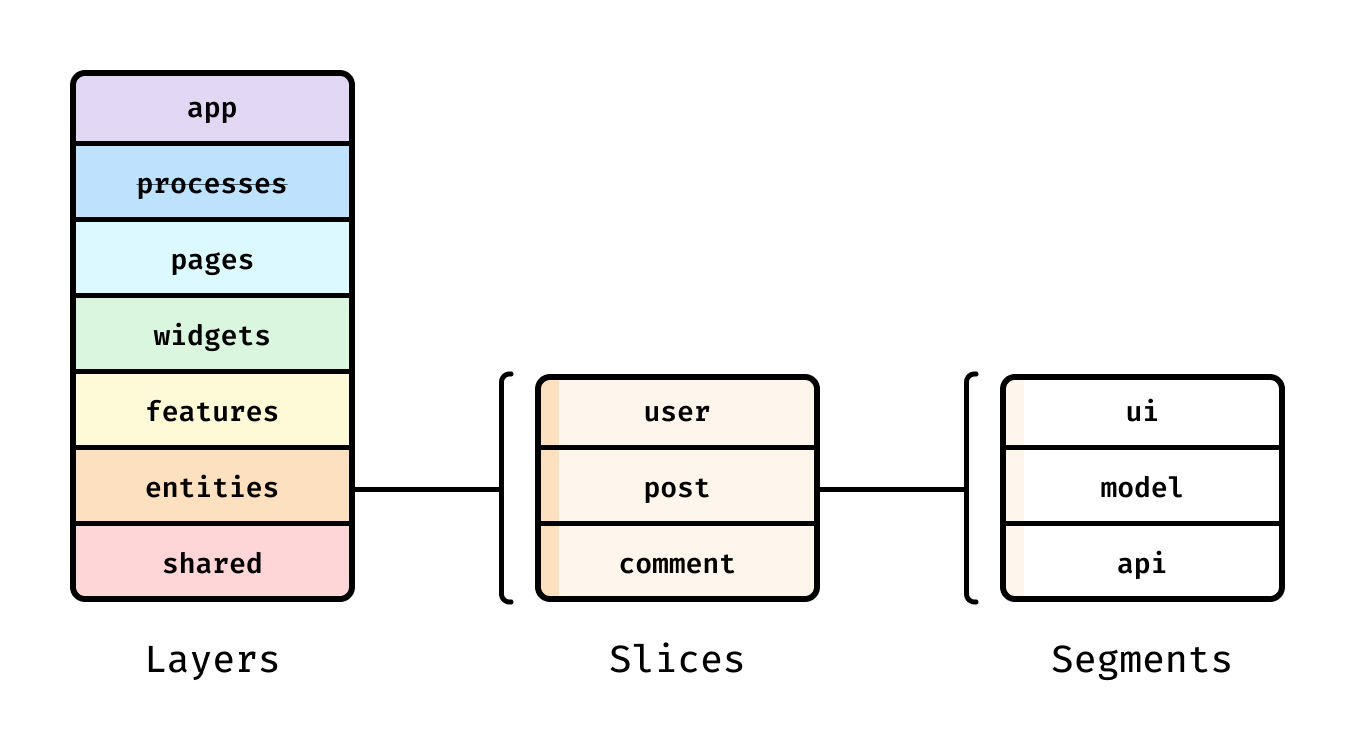
\includegraphics[width=0.7\linewidth]{static/fsdImage}
  \caption{Схема архитектуры клиентской части (FSD + Next.js)}
\end{figure}

На диаграмме представлены основные уровни и элементы архитектуры приложения. Следует отметить, что каждый слой в данной структуре ориентирован на строгое разграничение ответственности. Компоненты нижних уровней не имеют информации о вышестоящих слоях, что позволяет реализовать принцип инверсии зависимостей и минимизировать связанность между модулями.

\subsubsection{Слои архитектуры Feature-Sliced Design}

В таблице \ref{tab:fsd-layers} представлены слои архитектуры Feature-Sliced Design, сгруппированные по уровню абстракции и ответственности.

\begin{table}[h]
  \centering
  \caption{Слои архитектуры Feature-Sliced Design}
  \label{tab:fsd-layers}
  \begin{tabular}{|p{3cm}|p{11cm}|}
    \hline
    \textbf{Слой} & \textbf{Описание и назначение} \\ \hline
    \textit{app}      & Точка входа в приложение: глобальные стили, маршрутизация, провайдеры состояния, интеграции с внешними сервисами. \\ \hline
    \textit{pages}    & Страницы, связанные с маршрутизацией. Формируются из виджетов и не содержат бизнес-логики. \\ \hline
    \textit{widgets}  & Крупные элементы интерфейса, отражающие пользовательские сценарии, например, чат, список заданий, панель управления. \\ \hline
    \textit{features}& Изолированные пользовательские функции, такие как авторизация, отправка сообщений или регистрация. Могут включать бизнес-логику и вызовы API. \\ \hline
    \textit{entities} & Базовые предметные сущности предметной области, включающие типы, схемы, API и UI-представление. \\ \hline
    \textit{shared}   & Универсальные компоненты, утилиты и типы, переиспользуемые во всём проекте. \\ \hline
  \end{tabular}
\end{table}

\subsubsection{Концепция срезов (slices)}

Ключевым элементом архитектурного подхода Feature-Sliced Design является понятие срезов (англ. \textit{slices}). Под срезом понимается логически обособленный модуль, реализующий завершённую часть функциональности приложения. Каждый срез может содержать собственные модели данных, визуальные компоненты, бизнес-логику, а также механизмы взаимодействия с внешними источниками данных.

Например:
\begin{itemize}
  \item \textit{features/login} — срез, реализующий сценарий авторизации пользователя;
  \item \textit{entities/task} — срез, содержащий всё, что связано с сущностью «задание»;
  \item \textit{widgets/ChatWindow} — срез, объединяющий функциональность и интерфейс чат-интерфейса;
  \item \textit{pages/home} — срез, реализующий главную страницу приложения.
\end{itemize}

\subsubsection{Горизонтальное деление на сегменты (segments)}

Каждый срез, независимо от своего уровня, может быть дополнительно разделён на сегменты (англ. \textit{segments}) — логические подкатегории, структурирующие содержимое среза по назначению кода. В отличие от слоёв, которые представляют вертикальную иерархию, сегменты формируют горизонтальное деление и обеспечивают внутреннюю организацию модулей.

Наиболее распространённые типы сегментов включают:
\begin{itemize}
  \item \textit{ui} — визуальные компоненты и стили, определяющие отображение данных;
  \item \textit{model} — модели данных, хранилища состояния, типизация и бизнес-логика;
  \item \textit{api} — функции для работы с внешними сервисами, включая описание типов запросов и маппинг ответов;
  \item \textit{lib} — вспомогательные функции и библиотеки, используемые в пределах данного среза;
  \item \textit{config} — конфигурационные файлы и переключатели функциональности.
\end{itemize}

\subsubsection*{Преимущества выбранного подхода}

Применение архитектуры Feature-Sliced Design в контексте разрабатываемого клиентского приложения позволило достичь следующих результатов:
\begin{itemize}
  \item Чёткое разграничение обязанностей между модулями и слоями,
  \item Улучшенная масштабируемость проекта без деградации структуры,
  \item Повышенная модульность, обеспечивающая лёгкость в тестировании и повторном использовании кода,
  \item Создание условий для быстрой и эффективной интеграции новых членов команды в разработку,
  \item Архитектура, ориентированная на задачи и бизнес-логику, а не на технические детали.
\end{itemize}

В совокупности данные свойства делают архитектурное решение устойчивым к росту функциональности, улучшая поддержку и развитие системы в долгосрочной перспективе.
\subsection{Проектирование интерфейсных подсистем и экранов}

Одной из ключевых задач при проектировании клиентской части является логическое и функциональное разделение интерфейса на подсистемы, каждая из которых реализует отдельный аспект пользовательского взаимодействия. Такое разделение позволяет обеспечить модульность, переиспользуемость компонентов и устойчивость к изменениям.

Проект разрабатывается в архитектуре Feature-Sliced Design, что накладывает дополнительную дисциплину на организацию экранов и компонентов: все подсистемы формируются из \texttt{entities}, \texttt{features}, \texttt{widgets} и собираются в \texttt{pages}, а общая инфраструктура — в слое \texttt{shared}.

\subsubsection{Выделение ключевых интерфейсных подсистем}

Клиентская часть разработанной платформы организована в виде набора функционально обособленных интерфейсных подсистем, каждая из которых отвечает за определённый аспект пользовательского взаимодействия и бизнес-логики. Такое разграничение позволяет повысить масштабируемость и сопровождаемость системы, а также упростить процесс тестирования и внедрения новых функций.

На основании анализа требований к функциональности приложения и сценариев использования пользователями различных ролей (администратор, преподаватель, студент), были выделены следующие ключевые подсистемы.

\begin{enumerate}
  \item \textbf{Подсистема авторизации и регистрации}\\
  Отвечает за обеспечение безопасного входа в систему, регистрацию новых пользователей и управление сессиями. Аутентификация реализована с применением библиотеки \texttt{Auth.js} и технологии JSON Web Token (JWT), что позволяет надёжно разграничивать доступ к различным разделам интерфейса в зависимости от роли пользователя.  

  Регистрация в системе представлена в виде трёх пользовательских сценариев, адаптированных под особенности образовательного процесса:
  \begin{itemize}
    \item Первый сценарий реализован для новых организаций (институтов) и сопровождается созданием административной учётной записи. На этом этапе формируется корневая структура управления учреждением.
    \item Второй и третий сценарии предназначены для регистрации преподавателей и студентов соответственно. Оба сценария доступны исключительно по индивидуальным приглашениям, что обеспечивает контроль над составом участников образовательного процесса и предотвращает несанкционированный доступ.
  \end{itemize}
  
  Подсистема тесно связана с механизмами контроля прав доступа и маршрутизации, определяя поведение интерфейса в зависимости от текущего статуса пользователя.

  \item \textbf{Подсистема управления университетом}\\
  Реализует административную логику, связанную с конфигурацией организационной структуры образовательного учреждения (структура компонентов показана на Рис. \ref{fig:admin-components}).
  
  Основными функциями данной подсистемы являются:
  \begin{itemize}
    \item Создание и удаление структурных единиц — институтов, кафедр, учебных групп;
    \item Управление персоналом: добавление и блокировка преподавателей и студентов;
    \item Генерация приглашений для входа новых участников на платформу с конкретной ролью;
    \item Отображение данных по структуре учреждения.
  \end{itemize}
  
  Визуально подсистема представлена в виде панели управления с множеством таблиц, форм и интерактивных элементов, обеспечивающих быстрый доступ к ключевым административным операциям. Все действия защищены авторизацией и доступны только пользователям с соответствующими правами доступа.

  \item \textbf{Подсистема работы с заданиями и отправкой решений}\\
  Данная подсистема предназначена для организации учебной деятельности (структура компонентов представлена на Рис. \ref{fig:classroom-components}). 
  
  Основной интерфейс включает:
  \begin{itemize}
    \item Панель создания и редактирования заданий с параметрами проверки,
    \item Представление активных и завершённых заданий для студентов,
    \item Историю отправок с отображением результатов и статуса проверки.
  \end{itemize}
  
  Задания связаны с группами. Система также предоставляет базовую аналитику по результатам выполнения.

  \item \textbf{Подсистема обмена сообщениями (чаты)}\\ 
  В рамках образовательного процесса большое значение имеет возможность коммуникации (структура компонентов отображена на Рис. \ref{fig:chat-components}).
    
  \begin{figure}[H]
    \centering
    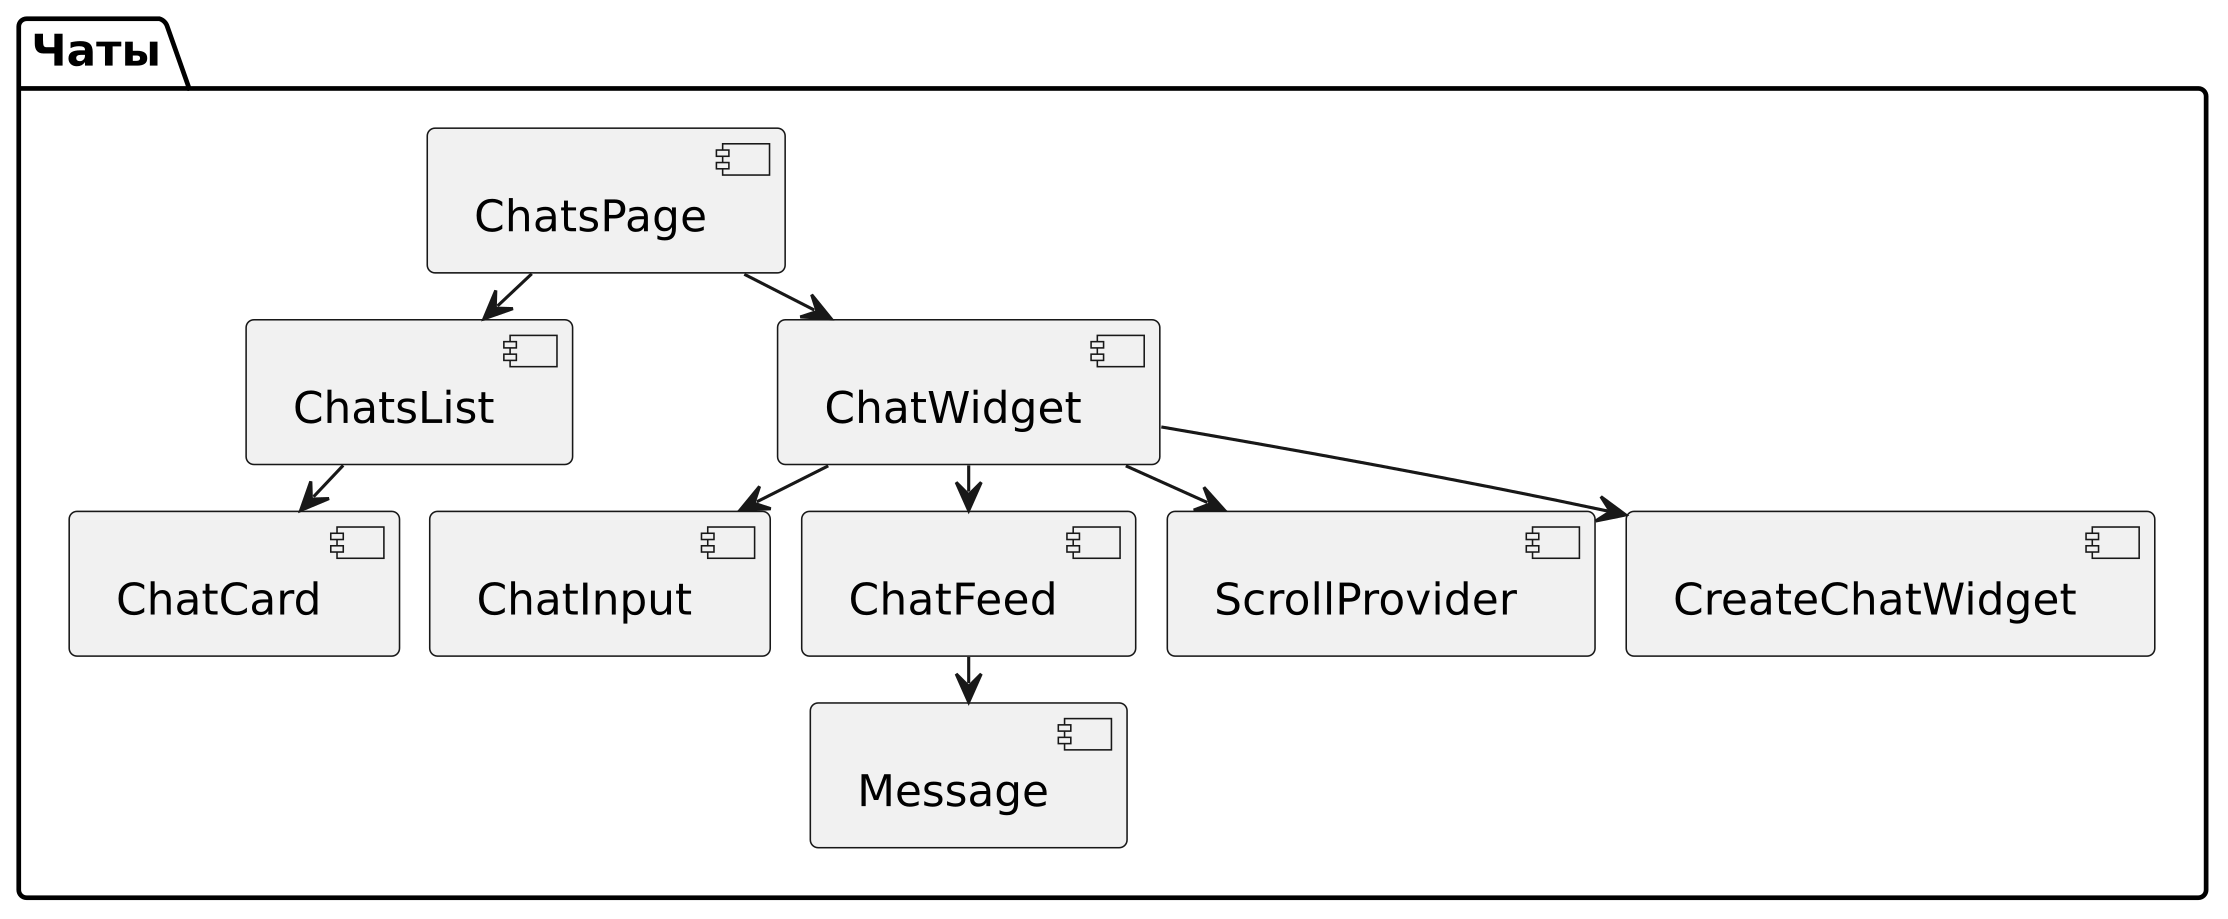
\includegraphics[width=0.9\textwidth]{static/diagrams/ChatsComponentDiagram.png}
    \caption{Диаграмма компонентов системы чатов}
    \label{fig:chat-components}
  \end{figure}
    
  Технически реализация основана на технологии WebSocket с использованием библиотеки \texttt{Socket.IO}, что обеспечивает мгновенную доставку сообщений и минимальную задержку при передаче данных.  
  
  Основной функционал включает:
  \begin{itemize}
    \item Подключение к соответствующим «комнатам» (группам или диалогам),
    \item Отправку и приём текстовых сообщений,
    \item Отображение истории переписки,
    \item Поддержку вложений и индикаторов прочтения.
  \end{itemize}
  
  Доступ к системе чатов осуществляется только после успешной авторизации, что исключает участие анонимных пользователей и обеспечивает безопасность переписки.

  \item \textbf{Подсистема AI-анализа решений}\\
  Одной из уникальных особенностей платформы является использование искусственного интеллекта для автоматической оценки студенческих заданий.
  
  Подсистема предназначена для получения и визуализации результатов AI-анализа, включающих:
  \begin{itemize}
    \item Оценку корректности кода;
    \item Проверку на соответствие заданию;
    \item Выявление потенциальных ошибок и некорректных конструкций;
    \item Комментарии, рекомендации и текстовые пояснения.
  \end{itemize}
  
  Результаты анализа отображаются в виде отчёта с возможностью преподавателя оставить дополнительные замечания. Таким образом, снижается нагрузка на преподавателя и повышается объективность оценивания.

\end{enumerate}

Каждая из указанных подсистем обладает чётко определёнными входными и выходными данными, а также взаимодействует с другими модулями системы. Например, подсистема работы с заданиями напрямую связана как с AI-анализом, так и с интерфейсами преподавателя и студента, а система чатов — с механизмами авторизации и маршрутизации. Такое проектирование обеспечивает гибкость, надёжность и чёткую масштабируемость клиентской архитектуры.

\subsubsection{Страницы и их структура}

Разработка интерфейсной части веб-приложения требует не только реализации функциональных компонентов, но и проектирования логически связанных экранов, отражающих ключевые сценарии взаимодействия пользователя с системой. В рамках платформы каждая страница представляет собой самостоятельный интерфейсный модуль, обслуживающий одну или несколько бизнес-задач, соответствующих определённой роли: студент, преподаватель, администратор.

Процесс формирования страниц реализован с применением маршрутизации, встроенной в фреймворк \texttt{Next.js}, что обеспечивает высокую производительность и поддержку серверного рендеринга. Страницы не только представляют визуальный уровень приложения, но и координируют работу между компонентами пользовательского интерфейса, бизнес-логикой и хранилищем состояния. 

Архитектурно страницы собираются из обособленных функциональных элементов, разработанных согласно принципам FSD: пользовательские действия реализуются в слое \texttt{features}, отображаемые сущности формируются на базе \texttt{entities}, а объединение этих блоков происходит внутри \texttt{widgets}. Такой подход позволяет повысить согласованность, переиспользуемость и модульность кода, а также снижает зависимость между различными частями интерфейса.

Ниже приведён перечень ключевых страниц, отражающих основную логику пользовательского взаимодействия.

\begin{itemize}
  \item \textbf{Страница авторизации}\\  
  Отвечает за вход пользователя в систему. Содержит форму для ввода учётных данных, а также реализует логику валидации, передачи данных на сервер, обработки ошибок и сохранения сессионного токена. После успешной авторизации пользователь перенаправляется на главную страницу, соответствующую его роли.

  \item \textbf{Страница заданий}\\
  Представляет собой ключевой интерфейс для организации и выполнения учебной деятельности. Интерфейс страницы включает:
  \begin{itemize}
    \item Список классов и учебных групп, к которым привязан пользователь,
    \item Перечень активных заданий в рамках каждой группы,
    \item Доступ к подробному описанию заданий, срокам сдачи и параметрам оценивания,
    \item Отправку решений и просмотр результатов, включая отчёты AI-анализа.
  \end{itemize}
  Для преподавателя дополнительно предоставляется интерфейс управления заданиями, а также доступа к аналитике по группам и студентам.

  \item \textbf{Административная панель института}\\
  Данная страница является основным рабочим инструментом пользователя с ролью администратора. Интерфейс включает:
  \begin{itemize}
    \item Управление иерархией образовательного учреждения (институты, кафедры, группы);
    \item Назначение и блокировка пользователей (студентов и преподавателей);
    \item Просмотр структуры учреждения в табличной форме;
    \item Генерацию и отправку приглашений на регистрацию;
    \item Журнал событий и контроль активности пользователей.
  \end{itemize}
  Все действия на данной странице требуют повышенного уровня доступа и сопровождаются системой уведомлений о результатах операций.

  \item \textbf{Страница чатов}\\
  Реализует коммуникационную составляющую платформы. Пользователь получает доступ к:
  \begin{itemize}
    \item Перечню активных диалогов (личных и групповых),
    \item Истории сообщений в рамках выбранного чата,
    \item Форме для отправки сообщений и файлов,
    \item Интерактивным элементам: индикаторы доставки, статус прочтения, поиск по переписке.
  \end{itemize}
  Для преподавателей также предусмотрена возможность создания новых групповых чатов для своих учебных групп.
\end{itemize}

Все функциональные страницы приложения, за исключением экранов регистрации и входа, используют единый шаблон компоновки \texttt{AppLayout}, обеспечивающий целостность визуального восприятия и унификацию пользовательского опыта. Данный шаблон включает в себя общие элементы интерфейса — верхнюю панель навигации, боковое меню и основной контейнер для отображения содержимого, который динамически наполняется в зависимости от текущего маршрута. 

Использование общего каркаса позволяет сохранить структурную согласованность между различными разделами системы, облегчает адаптацию пользователей к интерфейсу и упрощает внедрение изменений. Кроме того, архитектурное разделение логики и представления на уровне страниц способствует инкапсуляции ответственности, а также повышает читаемость и сопровождаемость кода. В рамках маршрутизации обеспечивается централизованное управление доступом, фильтрацией и визуализацией данных с учётом ролей пользователей.

Таким образом, структура страниц приложения отражает как технические требования архитектуры, так и практическую ориентацию на удобство и эффективность работы конечных пользователей.

\subsubsection{Компоненты и принципы их структурирования}

Компонентная модель проекта выстроена на основе принципов повторного использования, инкапсуляции и чёткого разделения ответственности между уровнями абстракции. Все компоненты, применяемые в рамках клиентского интерфейса, условно делятся на два основных класса: общие (универсальные) и специфические (бизнес-ориентированные).

\begin{itemize}
  \item \textbf{Общие компоненты} (\texttt{shared/ui}) представляют собой переиспользуемые элементы пользовательского интерфейса, не зависящие от предметной области. К ним относятся кнопки, поля ввода, модальные окна, индикаторы загрузки, элементы навигации, уведомления и другие базовые визуальные элементы. Такие компоненты широко применяются на всех уровнях интерфейса и не содержат бизнес-логики.
  
  \item \textbf{Специфические компоненты}, разрабатываемые в слоях \texttt{entities} и \texttt{widgets}, предназначены для реализации прикладной логики и отображения конкретных сущностей системы. Примерами являются компоненты отображения сообщений в чате, карточек заданий, панели управления преподавателя, таблиц пользователей и др. Они обладают внутренним состоянием и часто включают обращение к хранилищу или API.
\end{itemize}

Такое структурное разграничение существенно упрощает масштабирование проекта, облегчает поддержку и повторное использование элементов, а также способствует разделению труда между разработчиками.

\subsubsection{Распределение логики по слоям архитектуры}

Функциональная логика клиентской части системы строго распределяется по слоям архитектуры Feature-Sliced Design, что обеспечивает высокую модульность и инкапсуляцию поведения. Каждому слою соответствует свой уровень ответственности:

\begin{itemize}
  	\item В слое \texttt{entities} сосредоточена модель предметной области: типизация, структура сущностей, атомарные компоненты отображения, такие как \texttt{Registration}, \texttt{Department}, \texttt{Group}. Данный слой реализует описание и базовое представление данных без привязки к конкретным действиям пользователя.
  
	\item Слой \texttt{features} содержит реализацию отдельных действий, составляющих пользовательские сценарии: отправка сообщений, регистрация, загрузка задания, подтверждение действия и т.д. Эти модули инкапсулируют конкретные шаги взаимодействия пользователя с интерфейсом, часто включая локальное состояние и вызовы к API. \texttt{Features} могут быть использованы многократно и комбинироваться для построения более сложных сценариев.
	
	\item Слой \texttt{widgets} представляет собой реализацию полноценных пользовательских сценариев — законченных интерфейсных блоков, решающих определённую задачу. Примеры: интерфейс чата, панель с заданиями, административный модуль управления группами. Каждый виджет объединяет несколько фич и сущностей, обеспечивая завершённую и логически связанную единицу поведения.
	
	\item Слой \texttt{pages} выполняет роль точки входа и финальной сборки пользовательских сценариев. Здесь происходит выбор и компоновка виджетов в зависимости от маршрута, роли пользователя и контекста сессии. Кроме того, на уровне страниц задаются глобальные обёртки, обеспечиваются ограничения доступа, инициализируются загрузки данных и подключаются необходимые провайдеры. Таким образом, \texttt{pages} являются связующим слоем между навигацией и пользовательским опытом.
\end{itemize}

Такое строгое распределение обязанностей по слоям позволяет исключить дублирование логики, минимизировать связанность между модулями и обеспечить чёткую иерархию ответственности.

\subsubsection{UX-решения и пользовательские сценарии}

Для повышения удобства и доступности платформы, особенно в условиях использования её разными категориями пользователей, были реализованы следующие решения в области пользовательского опыта (UX):

\begin{itemize}
  \item \textbf{Централизованная навигация} — через универсальный макет, включающий боковую и верхнюю панели, интерфейс остаётся единообразным и интуитивно понятным вне зависимости от текущего маршрута.
  \item \textbf{Toast-уведомления} — реализация мгновенной обратной связи при выполнении действий: успешная отправка формы, ошибка сети, получение новых сообщений;
  \item \textbf{Обработка пустых состояний и ошибок} — предусмотрены интерфейсы для ситуаций отсутствия данных, ошибок загрузки или недоступности сервера.
\end{itemize}

В результате, пользователь получает предсказуемый и непрерывный опыт взаимодействия с системой вне зависимости от своей роли и уровня подготовки.

\subsubsection*{Вывод}

Проектирование интерфейсной части приложения основывается на чётком структурном и функциональном разграничении компонентов, ориентированном на принципы модульности и масштабируемости. Использование архитектуры Feature-Sliced Design позволяет изолировать бизнес-логику, визуальные компоненты и маршрутизацию, что делает интерфейс легко расширяемым и сопровождаемым.

Реализованная организация интерфейса, объединяющая единый шаблон компоновки, повторно используемые компоненты и специфические бизнес-модули, способствует формированию целостного пользовательского опыта. Выбранные UX-решения обеспечивают удобство и логичность навигации, а также высокую отзывчивость системы при взаимодействии с пользователем.


Интерфейсная часть проекта построена на модульной архитектуре, основанной на бизнес-функциях. Подсистемы выделены логически, а их реализация изолирована в независимые модули, что повышает удобство поддержки, расширения и переиспользования компонентов.
\subsection{Проектирование взаимодействия с сервером и WebSocket}

Клиентская часть приложения активно взаимодействует с сервером для получения и отправки данных, а также поддерживает постоянное соединение с помощью WebSocket в рамках подсистемы обмена сообщениями. При проектировании механизма взаимодействия были учтены требования безопасности, стабильности соединения, обработки ошибок, а также необходимость автоматического обновления сессионных данных пользователя.

\subsubsection{Аутентификация и управление токенами}
Для обеспечения защищённого доступа к функциональности платформы используется система авторизации с применением JSON Web Token (JWT). Управление сессией пользователя реализовано через библиотеку \texttt{Auth.js}, которая выполняет роль промежуточного слоя между клиентом и системой хранения токенов.

\begin{enumerate}
  \item \textbf{Аутентификация пользователя}:
  \begin{itemize}
    \item пользователь выполняет вход с помощью логина/пароля или через OAuth-провайдеров (например, Google);
    \item Auth.js инициирует процесс аутентификации и получает JWT при успешной проверке.
  \end{itemize}.
  
  \item \textbf{Работа с токеном}:
  \begin{itemize}
    \item полученный JWT содержит минимальный необходимый payload (например, идентификатор пользователя, роль и срок действия);
    \item токен сохраняется в \texttt{HTTP-only} cookie с флагами \texttt{Secure} и \texttt{SameSite=Strict}, что предотвращает XSS- и CSRF-атаки.
  \end{itemize}.
  
  \item \textbf{Доступ к защищённым ресурсам}:
  \begin{itemize}
    \item при обращении к API front-end автоматически прикрепляет токен к запросу;
    \item при недействительном или истёкшем токене Auth.js обновляет его через refresh-токен, если он присутствует.
  \end{itemize}.
\end{enumerate}

\subsubsection{Унифицированная функция отправки запросов}
Для стандартизации сетевого взаимодействия была разработана функция \texttt{sendRequest}, инкапсулирующая логику подготовки и отправки HTTP-запросов:
\begin{itemize}
  \item преобразование данных в JSON через \texttt{JSON.stringify};
  \item добавление заголовков, включая \texttt{Authorization: Bearer};
  \item обработка ошибок и повторная попытка после обновления токена;
  \item поддержка различных HTTP-методов.
\end{itemize}.

\subsubsection{Взаимодействие через WebSocket}
Для реализации обмена сообщениями в реальном времени используется библиотека \texttt{Socket.IO}, обеспечивающая:
\begin{itemize}
  \item автоматическое переподключение при обрыве соединения;
  \item передачу структурированных событий с именами и аргументами;
  \item интеграцию с middleware для авторизации;
  \item работу с пространствами имён и комнатами;
  \item fallback-транспорты при недоступности WebSocket.
\end{itemize}.

На стороне клиента реализован хук \texttt{useSocket}, который:
\begin{itemize}
  \item инициализирует соединение с сервером;
  \item отправляет и получает события с типизированными данными;
  \item подписывается и отписывается от каналов;
  \item управляет жизненным циклом подключения и логирует события;
  \item обрабатывает ошибки соединения.
\end{itemize}.

При установлении WebSocket-соединения клиент передаёт access-token в параметрах, сервер проверяет его и активирует соединение. В случае истечения срока действия токена:
\begin{enumerate}
  \item инициируется его обновление;
  \item текущее соединение закрывается;
  \item создаётся новое соединение с обновлённым токеном.
\end{enumerate}

\subsubsection*{Вывод}

Реализованные механизмы автоматического обновления токенов, единая функция отправки запросов и продуманная интеграция WebSocket через \texttt{Socket.IO} обеспечивают безопасность, надёжность и масштабируемость взаимодействия клиентской части с сервером в режиме реального времени.

\subsection{Интеграция ИИ-модуля DeepSeek в архитектуру проекта}

Для обеспечения эффективной работы ИИ-компонента в образовательной платформе реализована модульная архитектура с чётким разделением ответственности. Последующие подразделы детализируют ключевые аспекты интеграции: стратегию контейнеризации для изоляции сервиса, механизмы взаимодействия с клиентской частью и системные преимущества выбранного подхода. Основное внимание уделено сохранению прозрачности работы ИИ для конечных пользователей при обеспечении гибкости разработки и эксплуатации.

\subsubsection{Контейнеризация DeepSeek}
Для обеспечения независимого жизненного цикла и лёгкой масштабируемости ИИ-компонента DeepSeek развёртывается в виде изолированного Docker-контейнера. Такой подход позволяет:

\begin{itemize}
  \item быстро запускать и останавливать сервис без влияния на основное приложение;
  \item поддерживать разные версии DeepSeek параллельно, экспериментируя с обновлениями моделей;
  \item мигрировать между хостами и облачными средами с минимальными изменениями конфигурации.
\end{itemize}

\subsubsection{Преимущества контейнеризированного подхода}
Контейнеризация DeepSeek даёт следующие ключевые плюсы:
\begin{itemize}
  \item \textbf{Изоляция нагрузки}: анализ кода выполняется в отдельном окружении, не влияя на отзывчивость интерфейса;
  \item \textbf{Горизонтальное масштабирование}: при большом числе запросов можно запускать несколько инстансов контейнера;
  \item \textbf{Упрощённое сопровождение}: обновление ИИ-компонента сводится к выпуску нового Docker-образа без правок во фронтенде;
  \item \textbf{Гибкость развертывания}: контейнеры можно запускать локально и в облаке с одинаковой конфигурацией.
\end{itemize}

\subsubsection{Взаимодействие клиентской части с DeepSeek}

Клиентская часть приложения, реализованная на React и Next.js, отправляет HTTP-запросы к back-end части Web-приложения при прикреплении решения задания студентом, далее back-end автоматически начинает проверку решения при помощи AI-анализа. Результат проверки приходит пользователю при запросе на получения детальной информации по задаче, выполненной студентом.

\begin{figure}[H]
    \centering
    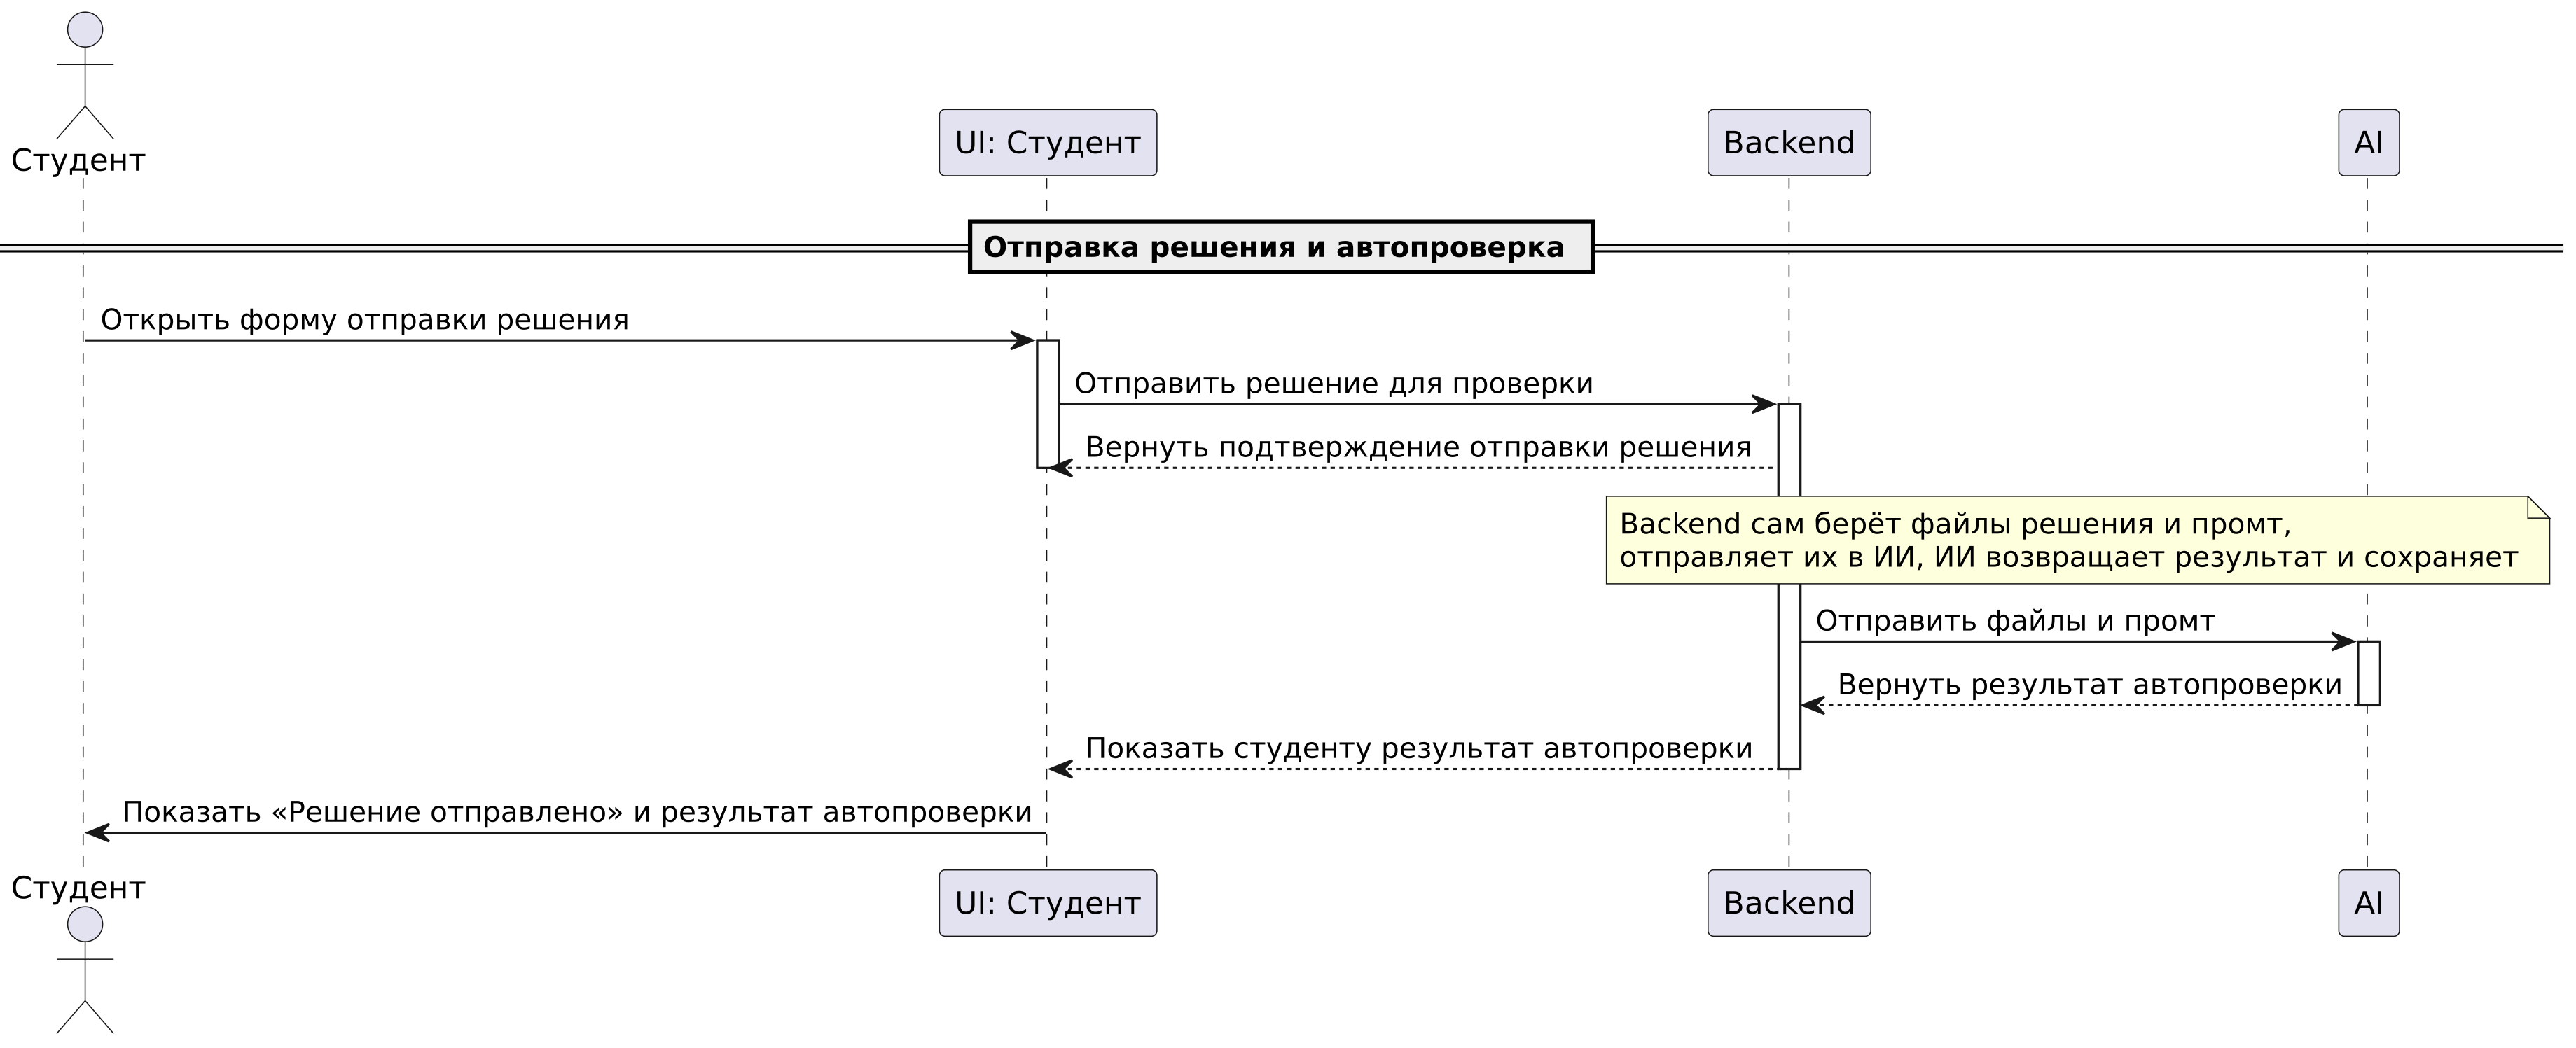
\includegraphics[width=0.8\linewidth]{static/diagrams/TaskSendStudentDiagram.png}
    \caption{Схема взаимодействия клиентской части (React/Next.js) с модулем DeepSeek}
    \label{fig:client-deepseek}
\end{figure}

На рисунке \ref{fig:client-deepseek} представлена схема взаимодействия клиентской части с модулем DeepSeek.

\subsubsection{Вывод}

Контейнеризация DeepSeek обеспечивает полную независимость остальных компонентов приложения от ИИ-модуля, позволяя развёртывать и обновлять его без влияния на другие сервисы. Взаимодействие через API бэкенда создаёт своего рода «чёрный ящик» для клиента, что упрощает инкапсуляцию логики и даёт гибкость в распределении и масштабировании нагрузки на контейнер с AI.



\subsection{Обеспечение безопасности клиентской части}

Безопасность пользовательского взаимодействия является важнейшей составляющей архитектуры клиентской части платформы. В условиях, когда доступ к различным модулям приложения осуществляется на основе ролей, а взаимодействие с данными сопровождается отображением пользовательского контента, особое внимание уделяется как управлению доступом, так и защите от потенциальных атак, включая межсайтовое выполнение скриптов (XSS). В данной подсистеме реализован комплекс механизмов, направленных на защиту данных и поведения интерфейса со стороны клиента.

\subsubsection{Разграничения доступа}
Одним из ключевых компонентов обеспечения безопасности клиентской части является система контроля доступа на основе промежуточного слоя — промежуточное программное обеспечение~\cite{nextjs_middleware}. В рамках архитектуры \textit{Next.js}, промежуточное программное обеспечение представляет собой функцию, исполняемую при каждом запросе к защищённым маршрутам. Она позволяет перехватывать обращения к страницам до их рендеринга и на этой стадии выполнять необходимые проверки: наличие токена, его валидность, а также права пользователя.

В контексте реализуемой платформы при обращении пользователя к любой защищённой странице клиентская логика через промежуточное программное обеспечение извлекает JWT-токен из cookies и дешифрует его содержимое, получая полезную нагрузку — уникальный идентификатор, срок действия сессии и роль в системе (\textit{admin}, \textit{teacher}, \textit{student}).

На основе этой информации промежуточное программное обеспечение выполняет следующие действия:
\begin{itemize}
  \item Если пользователь не авторизован (отсутствует валидный токен) — происходит автоматический редирект на страницу входа.
  \item Если пользователь авторизован, но не обладает достаточными правами — осуществляется перенаправление на главную страницу или отображается сообщение об отказе в доступе.
  \item Если пользователь обладает необходимой ролью — доступ к ресурсу предоставляется, и страница загружается с соответствующим контентом.
\end{itemize}

Таким образом, промежуточное программное обеспечение дает надёжную фильтрацию обращений к различным частям интерфейса, предотвращая несанкционированный доступ и соблюдая политику разграничения прав.

\subsubsection{Роль и защита при работе с форматируемым текстом}
Дополнительным вектором потенциальной угрозы в клиентских приложениях является отображение форматируемого текста, особенно если пользователь имеет возможность редактировать его содержимое. В таких случаях возрастает риск внедрения вредоносных скриптов, замаскированных под обычный HTML.

Для решения данной задачи в проекте используется библиотека \textit{tiptap} — расширяемый редактор форматированного текста на основе \textit{ProseMirror}. Одним из ключевых преимуществ \textit{tiptap} является контроль над тем, какие HTML-теги и атрибуты допускаются к отображению. Таким образом, даже если пользователь попытается вставить опасный код, редактор удалит такие элементы на этапе парсинга.

Технически это реализуется следующим образом:
\begin{itemize}
  \item при вводе содержимого редактор не сохраняет «сырые» HTML-строки, а формирует безопасное представление согласно заданным схемам;
  \item при рендеринге текста из базы или состояния редактор отображает только те элементы, которые были описаны как допустимые;
  \item расширения (extensions), добавляемые к \textit{tiptap}, позволяют точно контролировать список разрешённых тегов и атрибутов.
\end{itemize}

Таким образом, даже при наличии активной формы редактирования форматируемого текста пользовательская среда остаётся защищённой от внедрения опасного контента.

\subsubsection{Вывод}

Комплекс реализованных решений позволяет эффективно защитить клиентскую часть приложения как от внешнего вмешательства, так и от ошибочного доступа пользователей. Промежуточное программное обеспечение производит проверку сессии и прав доступа до загрузки страниц, а редактор \textit{tiptap} гарантирует безопасность при работе с форматируемым текстом. Такое сочетание архитектурных и прикладных средств создаёт устойчивую и безопасную пользовательскую среду.

\subsection{Покрытие бизнес-логики юнит-тестами}

Наш подход к обеспечению надёжности клиентского приложения фокусируется на обязательном юнит-тестировании бизнес-логики при помощи Jest. Тестирование UI-компонентов считается вторичным: написание и поддержка сравнений HTML-вывода часто оказывается более трудоёмким и хрупким, чем простая визуальная валидация. Визуальный осмотр интерфейса преподавателем или дизайнером даёт более быстрый и надёжный результат без лишних накладных расходов.

Основные принципы нашего подхода:
\begin{enumerate}
  \item Юнит-тесты покрывают функции, отвечающие за валидацию данных, расчёт оценок и другие критичные механизмы, гарантируя корректность работы независимо от изменений UI;
  \item Модульные тесты интерфейсов не используются: динамика верстки и частые мелкие правки приводят к избыточным провалам тестов и дополнительным усилиям на их поддержку;
  \item Благодаря отказу от snapshot-тестирования HTML структура текста программы остаётся гибкой, а команда освобождает время на развитие функциональности вместо постоянной правки тестов;
  \item Автоматический запуск тестов бизнес-логики при каждом пуше позволяет мгновенно обнаруживать регрессии и поддерживать стабильность продукта;
  \item Для окончательной валидации интерфейса используется ручной осмотр ключевых страниц после сборки, что даёт уверенность в корректности отображения без сложных технических средств.
\end{enumerate}

Такой подход обеспечивает надёжность самой логики приложения и упрощает работу с UI: вместо громоздких автоматизированных тестов на вёрстку мы применяем человеческую экспертизу для финальной проверки внешнего вида и пользовательского опыта.



\newpage
\ESKDthisStyle{formII}
\ESKDcolumnII{Список литературы}
\section{Список литературы}

\newpage

\ESKDthisStyle{formII}
\ESKDcolumnII{Приложения}
\section{Приложения}

\end{document}
